\subsection{Filter Design}

The typical Human can only hear frequencies in the range of 20Hz
through 20kHz, and this range only decreases as humans age
\cite{human:rg}. Using the website
\url{http://onlinetonegenerator.com/hearingtest.html}, we will
test the hearing range of each member listening to our final
presentation. This demonstration will provide a tangible example
why appropriate filtering of an audio signal will have little to
no impact on the quality of sound that a person hears after the  
filtering.

When our project group performed the hearing test, the highest
audible frequency was 15kHz. Since our project group was not able
to hear the frequencies above the 15kHz threshold, any low-pass
filter that removed the high frequencies above 15kHz would have
no impact on the quality of the audio signal that we would hear.
Recall that removing the unecessary frequencies from an audio signal
transmission provides a few nice benefits such as the following:

\begin{enumerate}
\item It reduces the necessary power for transmission of the audio signal,
\item It reduces the necessary bandwidth for transmission.
\end{enumerate}

Filtering is the processing of a time-domain signal resulting in
some change in that signals original spectral content. The change
is usually the reduction or filtering of unwanted input spectral
components\cite{lyons:intro}. Given the human threshold for
hearing, an obvious opportunity is to apply low-pass filtering in
order to transmit audio signals that humans can actually hear
with smaller bandwidths. The ideal low-pass filter would
completely eliminate all frequencies above a certain cutoff point
(in our hearing test example, the cutoff would be at 15kHz) while
passing all frequencies below the cutoff point  
\cite{lowpass:wiki}.

\begin{figure}[h!]
	\centering
	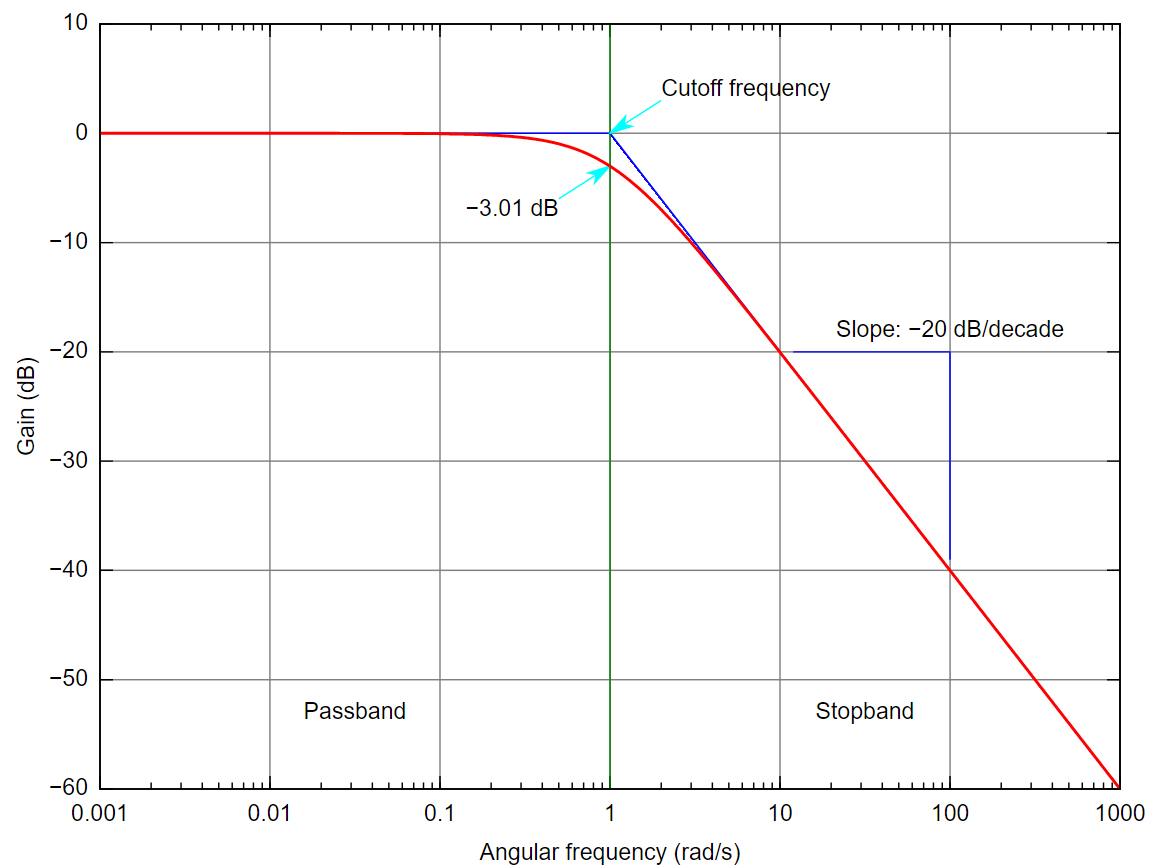
\includegraphics[scale = .5]{images/low_pass.png} %this is useful too \includegraphics[width = \linewidth]
	\caption{Example of Low-Pass Filter: \url{https://upload.wikimedia.org/wikipedia/commons/6/60/Butterworth_response.svg}}
	\label{fig:lowpass}
\end{figure}    

In order to filter out higher frequencies in an audio signal
transmission, we will build a low-pass filter. Specifically, we
will build a low-pass filter using a finite number of non-zero
filter coefficients which is called a \textit{Finite Impulse
Response} filter or FIR. Given an impulse response, we can find
the coefficients of the filter, and vice versa
\cite{notes:class}. For example, Figure \ref{fig:lowpass} shows a
graphical depiction of a low-pass filter that begins to cut out
the frequencies above 1 rad/s. Frequencies below the cutoff
frequency are considered to be in the
``passband," or allowable frequency band.  Frequencies above the cutoff frequency filtered out and are considered in the ``stopband."
Ideally, the slope between the passband and the stopband would be
as steep as possible to limit the passing of unwanted high audio
frequencies. The question still remains, how do you build a
filter that eliminates these frequencies? What is an impulse
response? How do we translate an impulse response to a frequency
response and vice versa. We address those questions next.

\subsubsection{Impulse Input, Impulse Response, and FFT}

 In our filtering example, we will be dealing with a linear
 time-invariant (LTI) System. A linear system is a class of
 systems where the system's outputs are the sum of the outputs of
 its parts. Additionally, time-invariant refers to a system
 where a time delay in the input sequence causes an equivalent
 delay in the output sequence. Now, if we are given a LTI system,
 we can calculate everything about the system if we know the
 \textit{unit impulse response}. The \textit{unit impulse
 response} refers to the system's time-domain output sequence
 when the input is a single unity-valued sample (unit impulse)
 surounded by zero-valued samples. Furthermore, knowing the
 impulse response of an LTI system, the \textit{output sequence}
 is calculated by taking the \textit{convolution} of the input
 sequence and the system's impulse response \cite{lyons:intro}.
 We will talk more about convolutions later, but we typically do
 not perform convolutions in the time domain since they are
 computationally expensive. Instead, multiplication is performed
 in the frequency domain. In order to transform the impuse
 response into a \textit{frequency response}, we take the Fast
 Fourier Transform (FFT) of the impulse
 response\cite{lyons:intro}.

Let's explain with a simple example. If we let $x(n)$ be a
discrete-time sequence of individual signal amplitudes, then we
can define a simple LTI \textit{averager} system that takes the
average of the last four inputs as follows:

$$y(n) = \frac{1}{4} \left[ x(n)+x(n-1)+x(n-2)+x(n-3)\right] =  \frac{1}{4}\sum_{k=n-3}^{n} x(k)$$    

Given this simple averager, we can show the block diagram in
Figure \ref{fig:impulse} (a), impulse input and impulse response
in Figure \ref{fig:impulse} (b), and the frequency magnitude
response created from the FFT of the impulse response in Figure
\ref{fig:impulse} (c). The block diagram in Figure
\ref{fig:impulse} (a) - also referred to as the \textit{filter
structure}, simply shows how an impulse input is transformed into
a impulse response. The impulse response, $y(n)$, is created by
passing the impulse input, $x(n)$, into the system and storing
the four most recent values. Once there are four values, they are
added together and multiplied by $\frac{1}{4}$ to calculate the
average. The sequence proceeds one step, and then performs
another average of the four most recent $x(n)$ values. The
averaging continues as long as impulse input enters the filter.
Since there are four separate input sample values to calculate an
output value, the structure of this filter can be referred to as
a \textit{4-tap tapped-delay line FIR filter} using digital
filter vernacular. The coefficients of this filter are all
$\frac{1}{4}$ and we can use an FFTon the filter to provide all
the frequency domain information.

For example, we can create a simple input impulse in Python by
generating random values between $-0.5$ and $0.5$ and then using
the numpy package in Python to apply the FFT in order to get the
frequency response, labeled x\_spectrum in Listing
\ref{lst:codedirect}, of the impulse input. We can then take get
the frequency response of the filter coefficients (labeled h\_n
in Listing \ref{lst:codedirect}) by performing another FFT. The
frequency response of the filter coefficients is labled as
freq\_response in Listing \ref{lst:codedirect}. Finally, we can
generate the new output spectrum by multiplying the x\_spectrum
and the freq\_response since they are both in the frequency
domain. See the entire code snipit below in Listing
\ref{lst:codedirect}. All of the code for this example to include
the code for the plots is listed in the Appendix.  

\lstset{language=Python}
\lstset{frame=lines}
\lstset{caption={Simple Averager Filter}}
\lstset{label={lst:codedirect}}
\lstset{basicstyle=\footnotesize}
\begin{lstlisting}
#generate impulse input
num_samples = 100
x_n = np.random.rand(num_samples)

#generate the frequency response for impulse input
X_m = np.fft.fft(x_n,N_fft)

#generate filter coefficients for simple averager
h_n = np.ones(4)/4

#generate the frequency response of the filter
# the second argument of fft is the number of fft bins

N_fft = 1024 #use a power of 2
H_m = np.fft.fft(h_n,N_fft)

#generate the output after filter
Y_m = H_m * abs(X_m)
\end{lstlisting}

Figure \ref{fig:exspec} shows the impact of the simple averager
filter on the original X\_m (input impulse after transformation
into the frequency domain). The original X\_m is ploted in blue
in the bottom graph in Figure \ref{fig:expec} and has a lot of
frequency information across the entire domain. Once the simple
average filter is applied, the output spectrum, Y\_m in red has
greatly reduced frequency content as the frequency gets further
away from 0. Additionally, you should notice that the output
spectrum (red line) is created by simply multiplying the
frequency response of the filter coefficients (top blue graph) by
the input spectrum (bottom blue graph).  

\begin{figure}[h!]
	\centering
	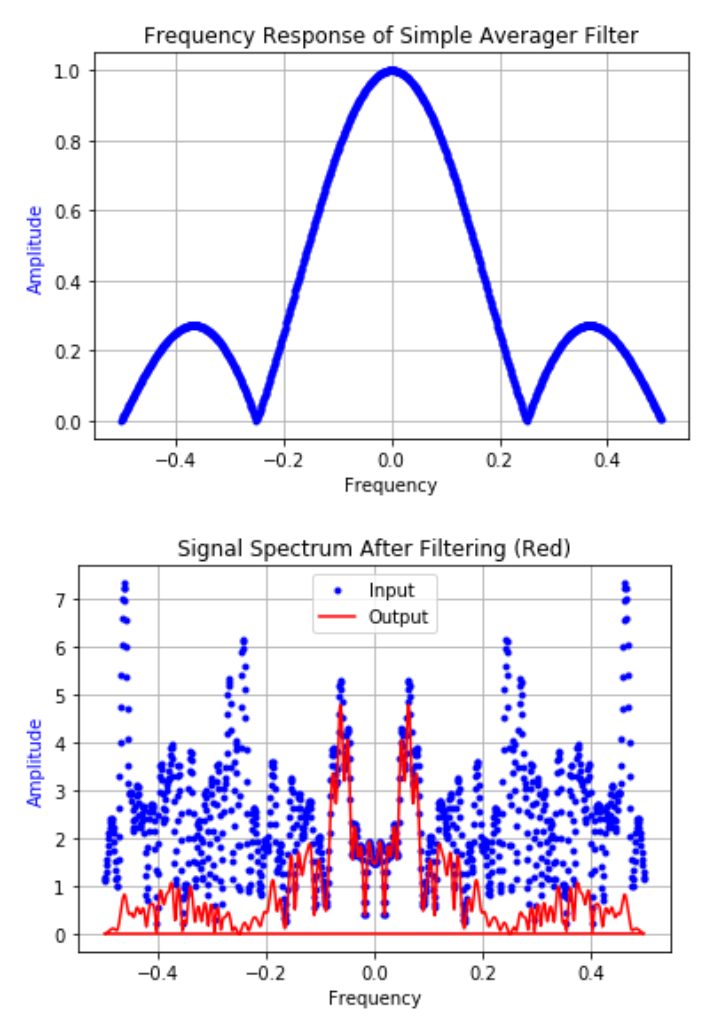
\includegraphics[scale = .8]{images/example_spectrum.png} %this is useful too \includegraphics[width = \linewidth]
	\caption{Frequency Response from the Filter Coefficients (TOP) and the Spectrum for Original Spectrum (blue) and Output Spectrum (red) after filter is applied (BOTTOM)}
	\label{fig:exspec}
\end{figure}    

The overview of this entire process is shown again in Figure
\ref{fig:impulse}. Looking at Figure \ref{fig:impulse} (c), the
FFT transforms the impulse response $y(n)$ into the frequency
information of $Y(m)$. $Y(m)$ provides the frequency magnitude
response after the filter has been applied to the impulse input
(also shown as the red line in the bottom graph of Figure
\ref{fig:exspec}). This is actually an example of a low-pass
filter where the \textit{averager} reduces the amplitude
(attenuates) of the high-frequency signal. In our construction of
a filter, we will have to use a different impulse response since
we want to remove, not attenuate, the high frequency information
content. The following section will explain how we design an FIR
filter using the FFT and inverse FFT.

\begin{figure}[h!]
	\centering
	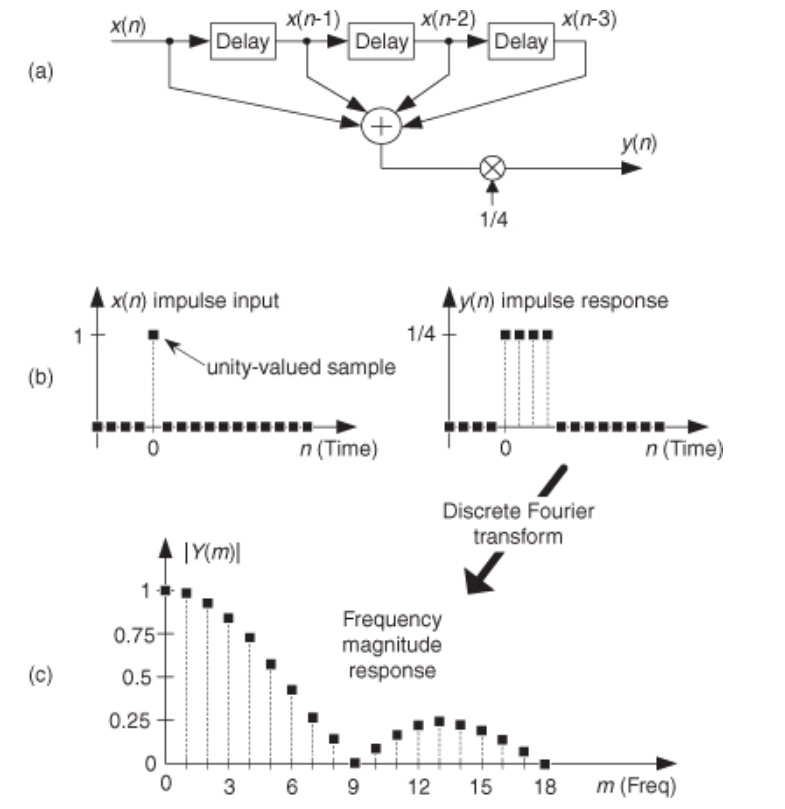
\includegraphics[scale = .6]{images/impulse.png} %this is useful too \includegraphics[width = \linewidth]
	\caption{Block Diagram (a), Impulse Input and Impulse Response (b), and Frequency Magnitude Response after FFT of Impulse Response (c).  Taken from Reference \cite{lyons:intro} below and is Figure 1-12 from Chapter 1}
	\label{fig:impulse}
\end{figure}   

\subsubsection{Finite Impulse Response (FIR)}

Now that we have laid down the groundwork with the general
overview and a simple example, we will discuss how to create an
FIR filter. An FIR filter has a finite duation of nonzero output
values given a finite duration of input values (this is how they
were named!). Recall, in our example above, we used four ``taps"
that were all equal to $\frac{1}{4}$. The two factors that affect
an FIR filter's frequency response are the number of taps and the
coefficients\cite{lyons:intro}. If we were to calculate the
impulse response, $y(n)$, from the impulse input, $x(n)$, in the
time-domain, then we would have to perform the mathematical
operation of a convolution. More specifically for an
\textit{M}-tap filter, we would calculate $y(n)$ as follows:

$$y(n) = \sum_{k=0}^{M-1}  h(k)x(n-k)$$

Where $h(k)$ are the filter coefficients for each of the taps.
\textbf{The terms FIR filter coefficients and impulse response
mean the same thing}\cite{lyons:intro}. We can re-write the above
equation using \textit{convolution} notation as follows:

$$y(n) = h(k) \star x(n)$$  

The major concept is that convolution in the time domain is equal
to multiplication in the frequency. The process in which we can
move from one domain by using an FFT. The FFT of $y(n)$ is equal
to $Y(m) = H(m) X(m)$, which is the spectrum of the filter
output. In our simple averager example above, we used
multiplication to create the blue line, $Y(m)$, in the bottom
graph of Figure \ref{fig:exspec}. In a similar way, we can
determine $y(n) = h(k)\star x(n)$ by taking the inverse FFT
(denoted as I-FFT) of $Y(m)$ \cite{lyons:intro} The FFT and the
inverse FFT allow us to move from the time domain to the
frequency domain, and from the frequency domain back to the the
time domain. To keep track of all the transformations, we listed
the important relationships are as follows: \\

\begin{enumerate}
\item $x(n) \overset{FFT}{\longrightarrow} X(m)$
\item $X(m) \overset{I-FFT}{\longrightarrow} x(n)$
\item $h(k) \overset{FFT}{\longrightarrow} H(m)$
\item $H(m) \overset{I-FFT}{\longrightarrow} h(k)$
\item $y(n) \overset{FFT}{\longrightarrow} Y(m) \Rightarrow h(k)\star x(n) \overset{FFT}{\longrightarrow} H(m) X(m)$
\item $Y(m) \overset{I-FFT}{\longrightarrow} y(n) \Rightarrow H(m) X(m) \overset{I-FFT}{\longrightarrow} h(k)\star x(n)$\\
\end{enumerate}    

The following section will explain how we design an FIR filter
using the GNU Radio Filter Design tool with the window method in
order to create a low-pass filter that removes high frequency
information content. The process ``behind the scenes" is similar
to the example with the simple averager.  

\subsubsection{GNU Radio: Filter Design Tool}

Now that we understand how to move between the frequency and
time-domains using the FFT or inverse FFT, let's design our own
low-pass filter by determining the desired frequency response and
moving back to the time domain through an inverse FFT to
calculate the filter coefficients that will provide the desired
frequency response. Recall, in our hearing test example, our
project group was unable to hear any frequency information
content above 15 kHz. As such, we will attempt to design a
low-pass filter that removes all of the frequency content above
this threshold. Therefore, our \textit{cutoff} frequency is 15kHz
(see Figure \ref{fig:lowpass} for a depiction of the cutoff
frequency). To design the filter, we define the \textbf{frequency
cut-off values} (end of passband and beginning of stopband), the
\textbf{sample rate}, and the \textbf{stopband attenuation} (in
decibels), and then use a Filter Design Tool within the GNU Radio
application (which is written in Python) to apply the inverse FFT
function to get the FIR filter coefficients.  

\begin{figure}[h!]
	\centering
	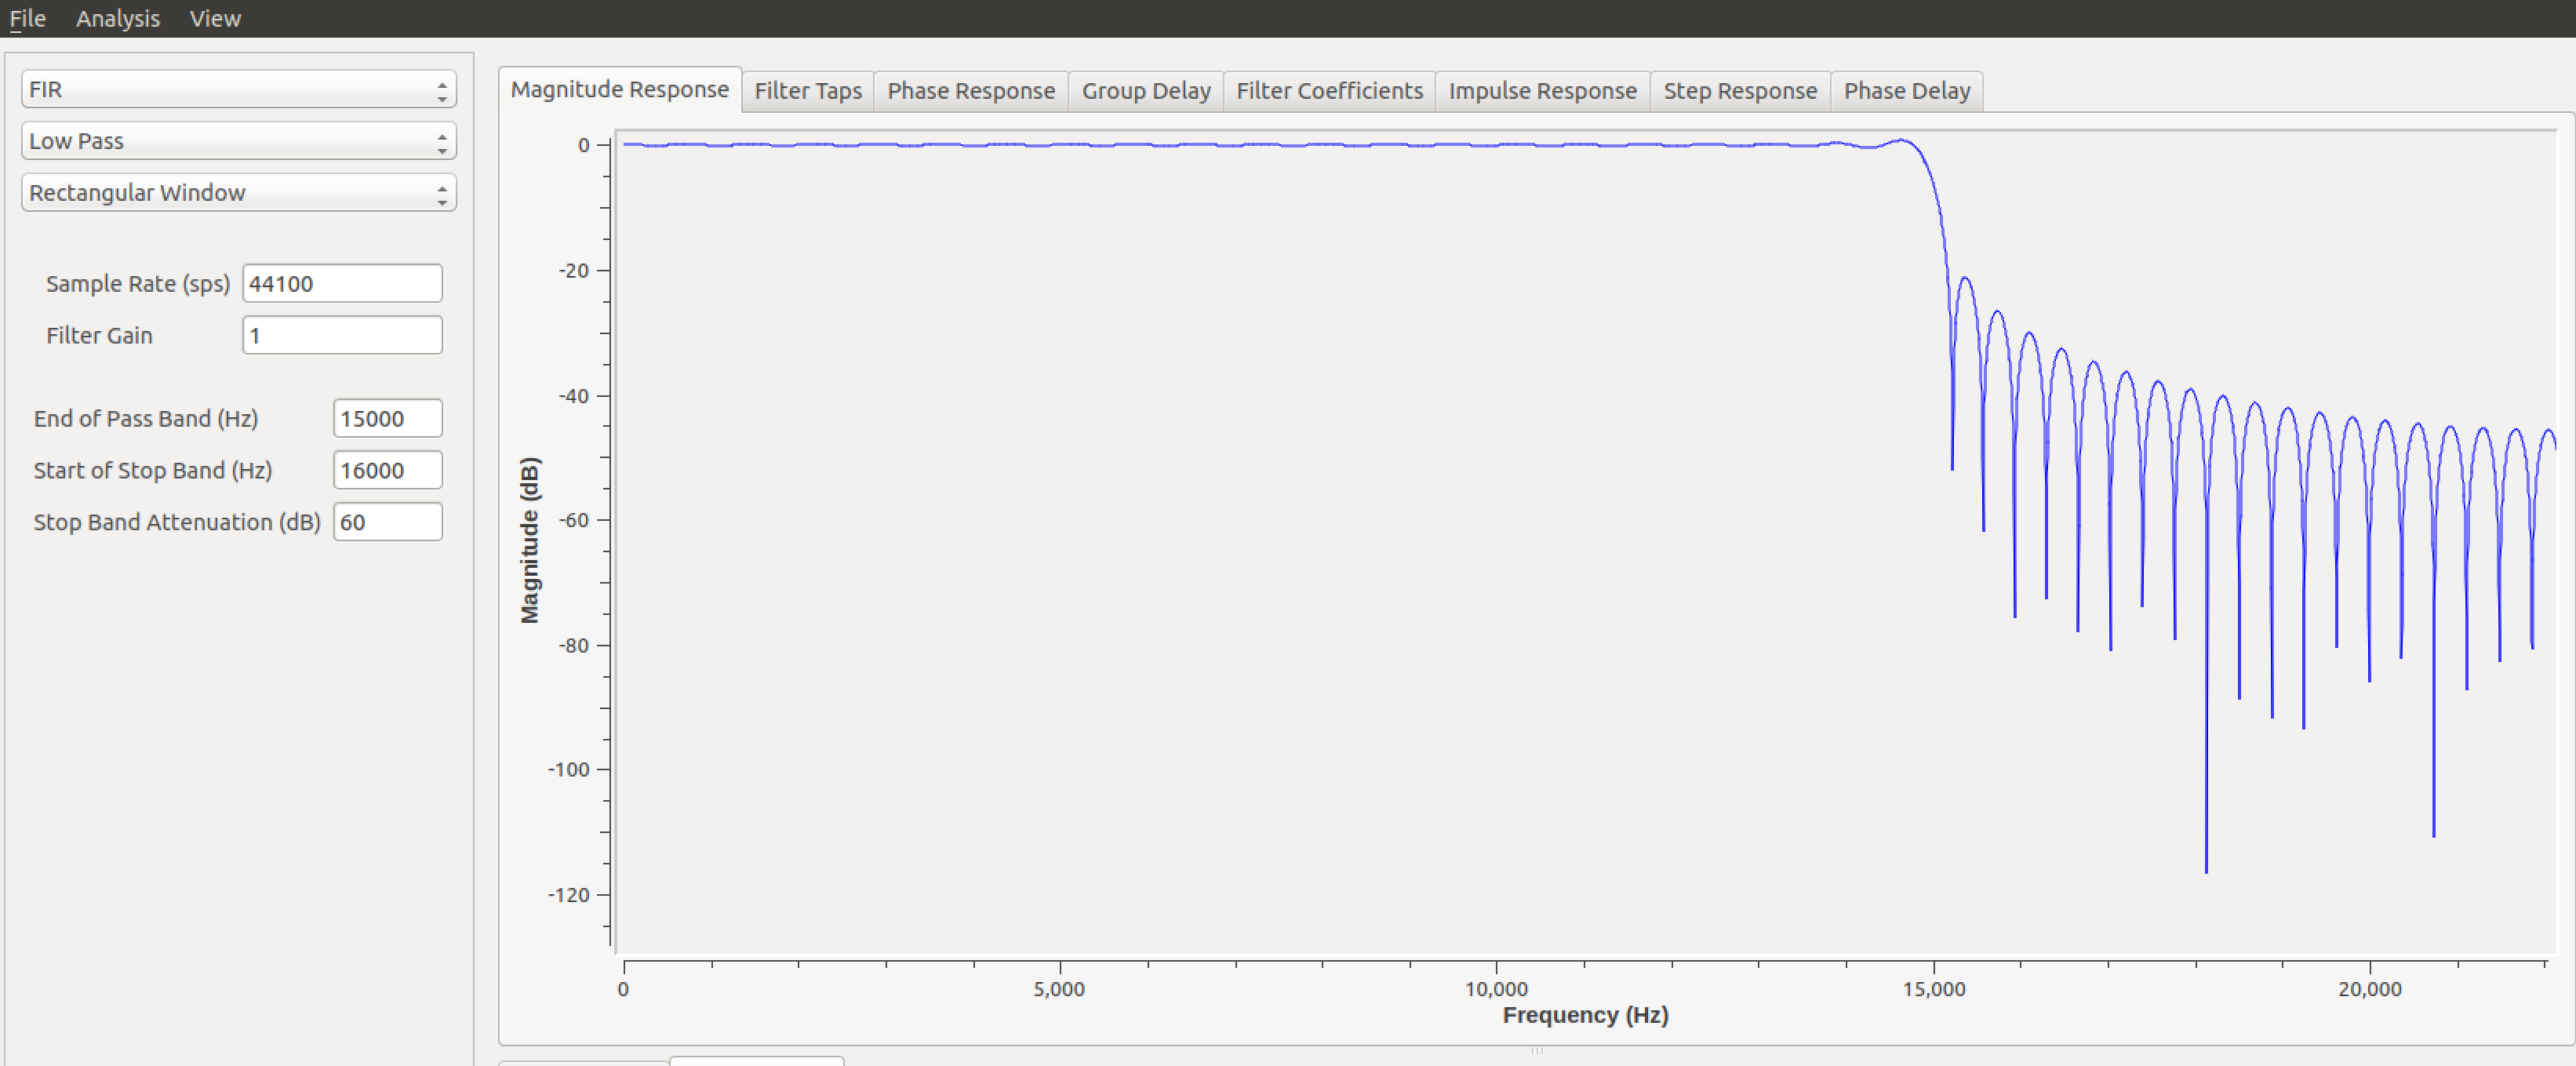
\includegraphics[height = 5cm, width =9cm]{images/filter_tool_15kHz.png} %this is useful too \includegraphics[width = \linewidth]
	\caption{Designing the 15 kHz Filter using the Filter Design Tool within GNU Radio}
	\label{fig:mainfilt}
\end{figure}  

We set the sample rate $= 44,100$, the end of the passband at
$15$ kHz, the beginning of the stopband at $16$ kHz, and the
stopband attenuation at $60$ dB. After hitting the ``Design"
button, the tool creates the frequency response for the desired
filter which is displayed in Figure \ref{fig:mainfilt}. As
expected, the frequency response shows a drop-off at 15 kHz where
the passband ends and the frequencies are cut. The tool will take
the inverse FFT of the frequency response in order to generate
the filter coefficients, or taps. Figure \ref{fig:taps15} shows
the filter coefficients that provide the frequency response that
removes frequency above 15 kHz. The filter coefficients are saved
and then passed into the GNU Radio Tool that implements the
filter created.  

\begin{figure}[h!]
	\centering
	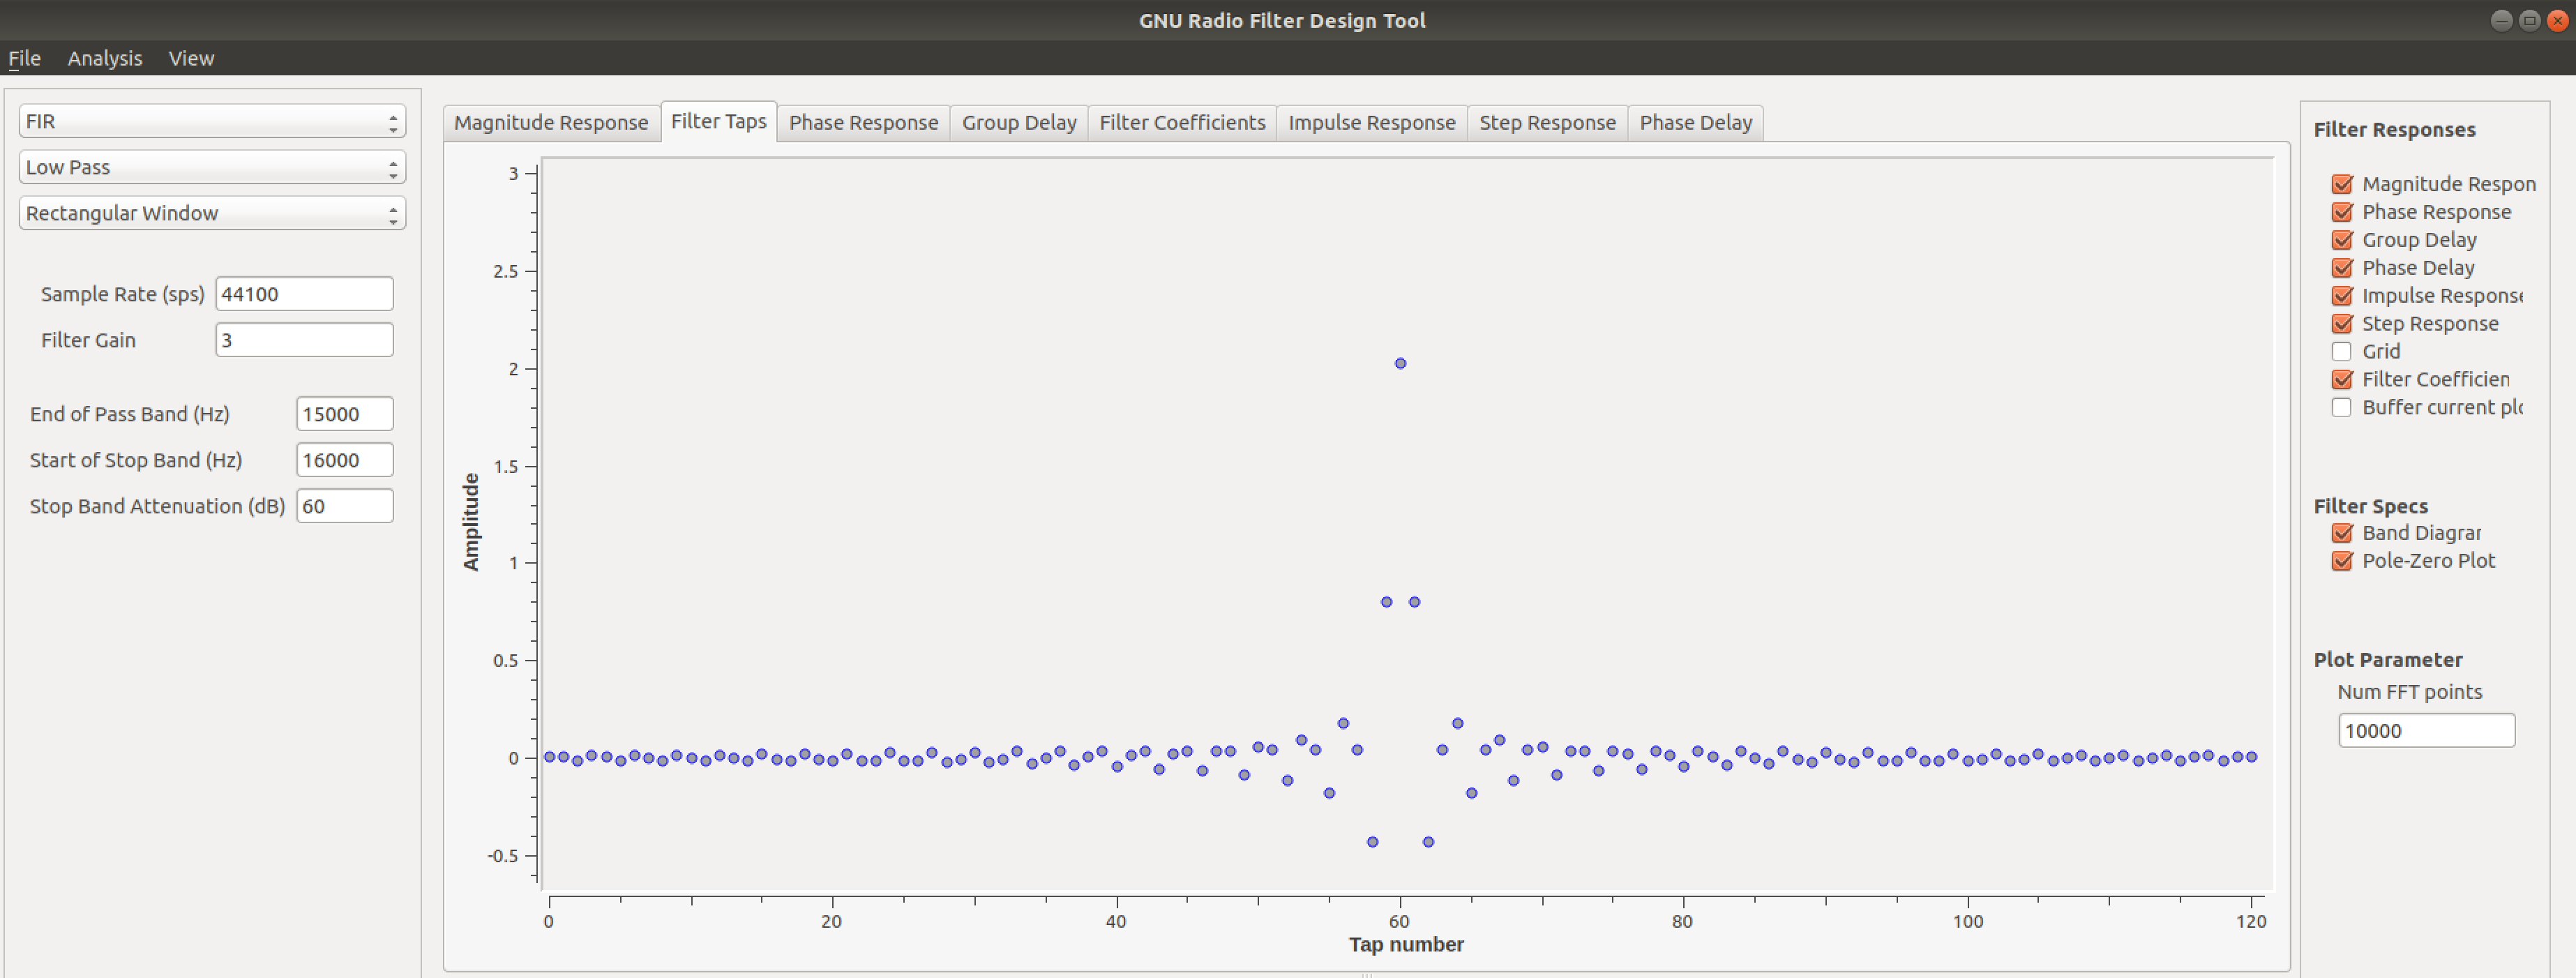
\includegraphics[height = 5cm, width =9cm]{images/filter_tool_15kHz_taps.png} %this is useful too \includegraphics[width = \linewidth]
	\caption{Filter Coefficients for the 15 kHz Filter using the Filter Design Tool within GNU Radio}
	\label{fig:taps15}
\end{figure}   
  
 
